\documentclass[a4paper]{article}
\usepackage[dutch]{babel}
\usepackage{amsmath}
\usepackage{graphicx, caption, lipsum}
\usepackage{lscape}
\captionsetup{belowskip=12pt,aboveskip=4pt}

\title{Practicum NMB : Practicum 1}
\author{Alexander Boucquey, Tristan Van Thielen}
\date{vrijdag 21 april 2017}

\newcommand{\opgave}[1]{\section*{Opgave #1}}
\newcommand{\dx}{\Delta x}
\newcommand{\dy}{\Delta y}
\newcommand{\dz}{\Delta z}
\newcommand{\dt}{\Delta t}

\begin{document}
\maketitle

\opgave{1}
Om de eigenvectoren en eigenwaarden van een Householdermatrix te bekijken is het nodig om te weten hoe deze wordt opgesteld. De transformatiematrix \textbf{Qk} is een combinatie van een (k-1)x(k-1) identiteitsmatrix en de (m-k+1)x(m-k+1) unitaire householdermatrix \textbf{F}. F wordt opgesteld  via:\\

$F = I -2(vv^{*})/(v^{*}v)$\\

In deze vorm is de projectiematrix $P = (vv^{*})/(v^{*}v)$ makkelijk herkenbaar. Het verschil is dat er dubbel zo ver geprojecteerd wordt. Het is mogelijk om van deze matrix de eigenwaardenontbinding op te schrijven:\\

\[
P = Q \Lambda Q^{T} = 
\begin{bmatrix}
    \vdots      & \vdots &  & \vdots\\
    v/\|v)\| & q_{2} & \dots & q_{n}\\
   \vdots      & \vdots &  & \vdots
\end{bmatrix}
\begin{bmatrix}
    -1\\
      & 1\\
      &   &  \ddots\\
	& & & 1
\end{bmatrix}
\begin{bmatrix}
    \vdots      & \vdots &  & \vdots\\
    v/\|v)\| & q_{2} & \dots & q_{n}\\
   \vdots      & \vdots &  & \vdots
\end{bmatrix}^{T}
\]\\

De vectoren $q_{2}$,...,$q_{n}$ vormen hier dan een orthonormale basis voor de (n-1) dimensionele deelruimte loodrecht op v. De vectoren q kunnen gevonden worden via Gram-Schmidt. Belangrijk is om nu in te zien dat $QQ^{T} = I$. Daardoor kan de formule voor F geschreven worden als:\\

$F = QQ^{T} - 2Q \Lambda Q^{T} = Q(I - 2\Lambda)Q^{T}$\\

In deze formule wordt duidelijk dat de eigenwaarden van F voldoen aan $\lambda_{i}(F) = 1-2\lambda_{i}(P)$. De reeks van eigenwaarden voor F is dus (-1, 1, 1, ..., 1). De eigenvectoren van F zijn dezelfde als deze van P en dus voldoen ze ook aan dezelfde eigenschappen. Omdat F reëel en symmetrisch is, voldoet deze ook aan de eigenschap dat al zijn eigenwaarden -1 of 1 zijn.



\opgave{2}
Wanneer we de tijdsduur berekenen van de gebruikte methode zien we dat het voor kleine matrices een klein verschil geeft, maar voor grote matrices het een grootteorde verschil is.\\[12pt]

\centering
\begin{tabular}{|r|c|c|c|}
\hline
Grootte van A & 10x10 & 100x100 & 1000x1000\\ \hline
Expliciet & 0.0022s & 0.0165s & 48.8148s\\ \hline
Impliciet & 0.0020s & 0.0082s & 4.3914s\\ \hline
\end{tabular}
\centering
\captionof{table}{Tijdsduur van Householder.}
\label{Tijd Householder}

\begin{flushleft}
Wanneer de fout (zowel op x als op het residu) nader bekeken wordt, blijkt deze nagenoeg hetzelfde te zijn. Het verschil in beide algoritmes bevindt zich dus in de tijdsduur, de impliciete berekening is dus de snelste. De resultaten van de fout zijn te vinden in bijlage 1.\\[12pt]
\end{flushleft}


\begin{flushleft}


\opgave{3}
De resultaten van deze vraag zijn te vinden in Bijlage 1. In deze tabel staan de coëfficiëntenvector x en het residu. Het is logisch dat het residu verkleint wanneer n stijgt. Er zijn meer vectoren u en dus is komt men steeds dichter bij een basis voor ${\rm I\!R}^{m}$. Het verhogen van n heeft steeds een kleiner effect, aangezien het bereik van alles vectoren samen slechts minimaal wordt vergroot. \\

In de resultaten is dit gedrag zeer herkenbaar. We zien dat vanaf n = 23 elke verhoging van n slechts een verschil maakt van ongeveer 0.1. Dit is merkbaar kleiner dan de stappen ervoor die een verschil van eenheden of zelfs tientallen teweegbrengen. Merk wel dat het residu nog steeds zeer groot is. Dit is omdat er nog steed veel te weinig vectoren zijn ivm. de dimensie van het probleem nl. 400. Voor een n = 200 wordt het residu veel kleiner. Dan zijn er immer veel meer vectoren om een lineaire combinatie van te maken.\\


\opgave{4}
De definitie van het Rayleigh quoti\"ent is:\\

$r(x) = \dfrac{x^{T}Ax}{x^{T}x}$

Bij eigenvectoren volgt hier een makkelijke omzetting:\\

\begin{equation}
\begin{gathered}
r(x) = \dfrac{v^{T}Av}{v^{T}v} = \dfrac{v^{T}\lambda v}{v^{T}v} = \lambda
\end{gathered}
\end{equation}

Volgens formule 27.2 uit Trefethen en Bau:\\

\begin{equation}
\begin{gathered}
\nabla r(x) = \dfrac{2}{x^{T}x}(Ax - r(x)x)
\end{gathered}
\end{equation}

Voor eigenvectoren wordt de term (Ax - r(x)x) = 0. Minima en maxima van het Rayleigh quoti\"ent liggen dus bij eigenvectoren. Uit (1) volgt dan dat de waarde hier gelijk is aan $\lambda$. Het maximum wordt dan bereikt bij $v_{max}$ en een minimum bij $v_{min}$. De waarden zijn daar $\lambda_{max}$ en $\lambda_{min}$.\\

Om het bewijs af te ronden is het nog nodig om te weten dat de eigenvectoren van A hier een orthonormale basis vormen voor de ruimte ${\rm I\!R}^{n}$. Alle vectoren kunnen dus voorgesteld worden als een lineaire combinatie van de eigenvectoren van A. Wanneer we dit combineren met de definitie van het Rayleigh quoti\"ent, vinden we:\\

\begin{equation}
\begin{gathered}
r(x) = \dfrac{\sum_{i=1}^{n}(\alpha_{i}v_{i})^{T}A\sum_{i=1}^{n}(\alpha_{i}v_{i})}{\sum_{i=1}^{n}(\alpha_{i}^{2}\|v\|^{2})} = \dfrac{\sum_{i=1}^{n}(\alpha_{i}^{2}\lambda_{i})}{\sum_{i=1}^{n}\alpha_{i}^{2}}
\end{gathered}
\end{equation}

De minimale waarde die kan bereikt worden is dus $\lambda_{min}$ en het maximum is $\lambda_{max}$. Uit (3) volgt ook meteen het bewijs voor het tweede deel. Elke waarde binnen het interval kan geschreven worden als een lineaire combinatie van eigenwaarden. Met deze co\"effici\"enten kan men dan de co\"effici\"enten bepalen voor de vector x als lineaire combinatie van eigenvectoren.\\

\opgave{5}
\subsection*{Vraag 5a}
QR en gelijktijdige iteratie berekenen alle eigenwaarden en bijhorende eigenvectoren. Gelijktijdige iteratie bij een vierkante matrix met Q(0) = I is hetzelfde als het QR algoritme zonder shift. Beide algoritme convergeren lineair.\\ [12pt]

Het QR algoritme met (RQ) shift gebruikt het principe van inverse iteratie. Dit berekent alle eigenwaarden.De Rayleigh Quot\"ent iteratie maakt ook gebruik van inverse iteratie en Rayleigh Quoti\"ent, om te convergeren naar de hoogste eigenwaarden. Beide laatste convergeren kubisch naar hun eigenwaarden.\\ [12pt]

Alle algoritmes, behalve de Rayleigh Quoti\"ent iteratie, berekenen alle eigenwaarden.\\ [12pt]

\subsection*{Vraag 5b}
Het QR-algoritme met RQ shift past de Rayleigh Quoti\"ent iteratie toe op alle vectoren tegelijk. Het gelijktijdig toepassen op een hele matrix is het gelijktijdige iteratie algoritme, de Rayleigh Quoti\"ent iteratie is wat er gebeurd op iedere vector.\\[12pt]

Wanneer naar het residu gekeken wordt zien we dat het Rayleigh Quoti\"ent in een drie stappen naar machine precisie convergeert. De gelijktijdige iteratie en QR zonder shift 35 iteratie stappen over het berekenen van alle eigenwaarden op machine nauwkeurigheid. QR met Rayleih Quoti\"ent shift convergeert even snel als het Rayleigh Quoti\"ent zelf, maar voor alle eigenwaarden.\\[12 pt]
\begin{center}
\makebox[\textwidth]{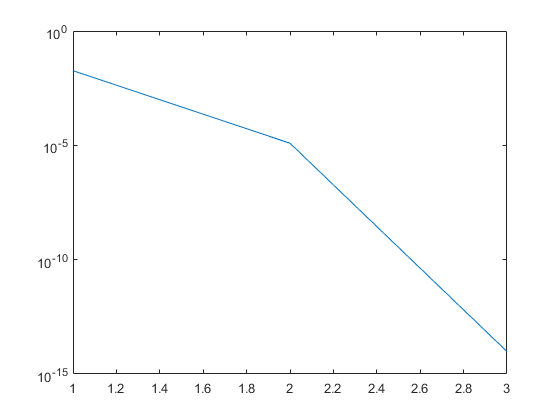
\includegraphics[width = \paperwidth, height=8cm]{Tekeningen/residu_rayleigh}}
\end{center}
\caption{Residu Rayleigh.}

\begin{center}
\makebox[\textwidth]{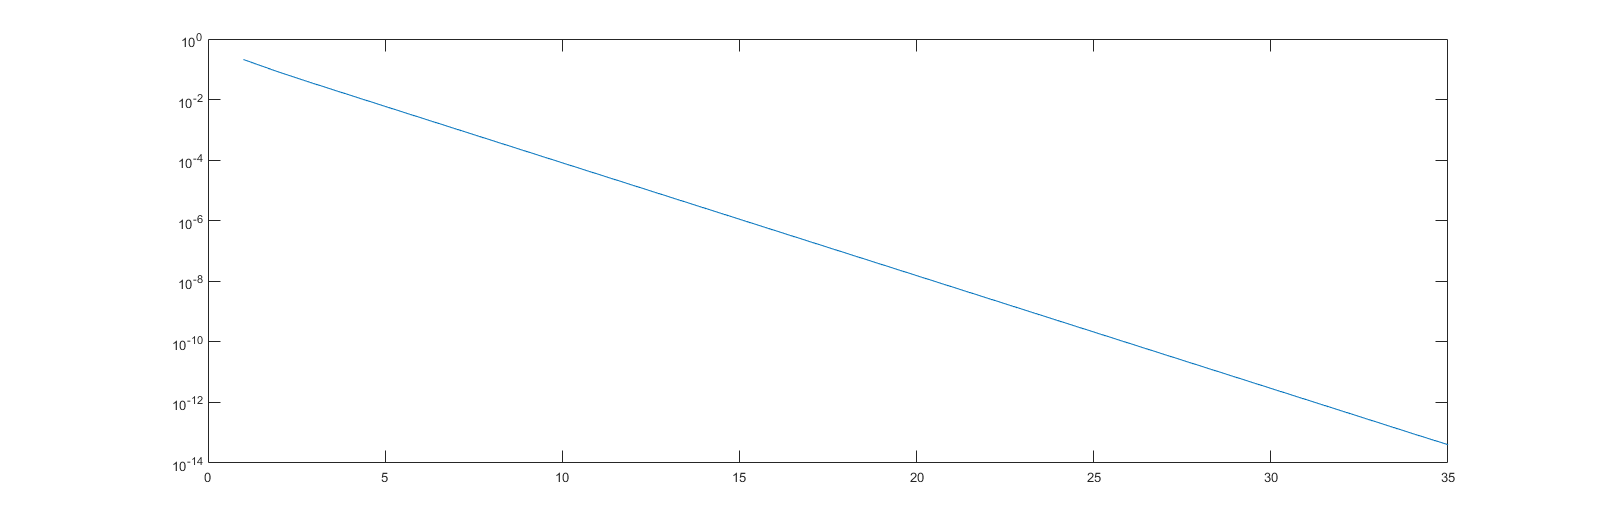
\includegraphics[width = \paperwidth, height=8cm]{Tekeningen/residu_gelijktijdige_it_randomQ}}
\end{center}
\caption{Residu gelijktijdige iteratie.}

\begin{center}
\makebox[\textwidth]{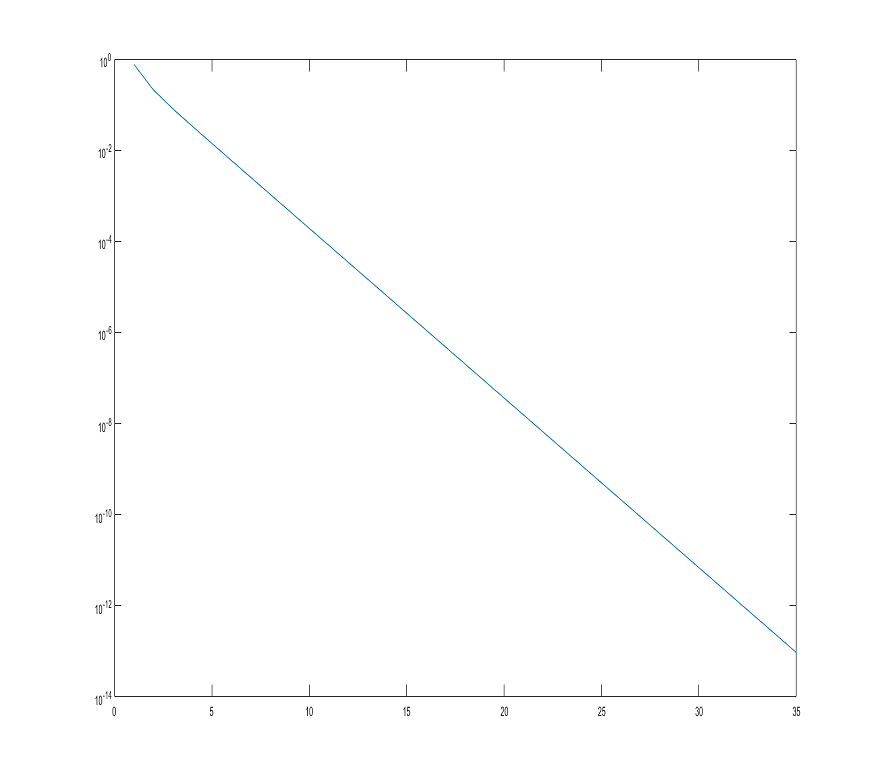
\includegraphics[width = \paperwidth, height=8cm]{Tekeningen/residu_qr_zonder}}
\end{center}
\caption{Residu QR algoritme zonder shift.}

\begin{center}
\makebox[\textwidth]{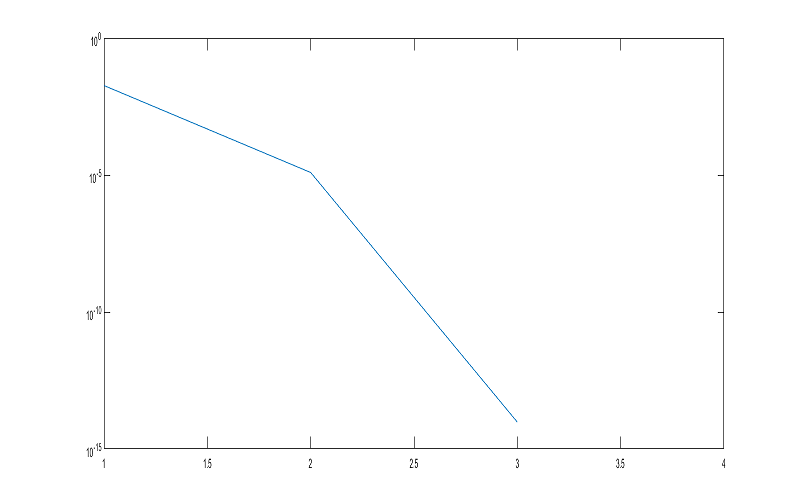
\includegraphics[width = \paperwidth, height=8cm]{Tekeningen/residu_qr_shiftrayleigh}}
\end{center}
\caption{Residu QR algoritme met Rayhleigh shift.}





\opgave{6}
De grenzen voor de methode van geconjungeerde gradiënten worden gegeven door formule 38.10 uit Trefethen en Bau:\\

$\dfrac{\|e_{n}\|_{A}}{\|e_{0}\|_{A}} \leq 2(\dfrac{\sqrt{\kappa} - 1}{\sqrt{\kappa} + 1})^{n}$\\[12pt]

In de opgave is alles gegeven om met n = 10 het conditiegetal $\kappa$ te kunnen berekenen. Na omvorming van de formule vindt men dat $\kappa \geq 9$.
Nu deze ondergrens bekend is, kan men hieruit een nieuwe bovengrens afleiden voor de fout bij n = 20. Nogmaals na omvormen van de formules geeft dit als bovengrens $\|e_{20}\|_{A} \leq 1.9073*10^{-6}$.\\


\opgave{7}
Wanneer we het convergentie gedrag bekijken van de Ritz waarden valt op dat de meest extreme eigenwaarde (zie \ref{arnoldi_1_100_it}) het snelste convergeert. De andere eigenwaarde liggen dicht bij elkaar geclusterd en convergeren veel langzamer (bv. \ref{arnoldi_2_150_it} haalt na 150 iteraties nog altijd maar een precisie van $10^{-5}$, nog lagere extremen gaan uiteraard nog langzamer (\ref{arnoldi_3_150_it} en \ref{arnoldi_4_150_it}).
\begin{figure}[H]
  \centering
  \subfloat[arnoldi 1, 100 iteraties]{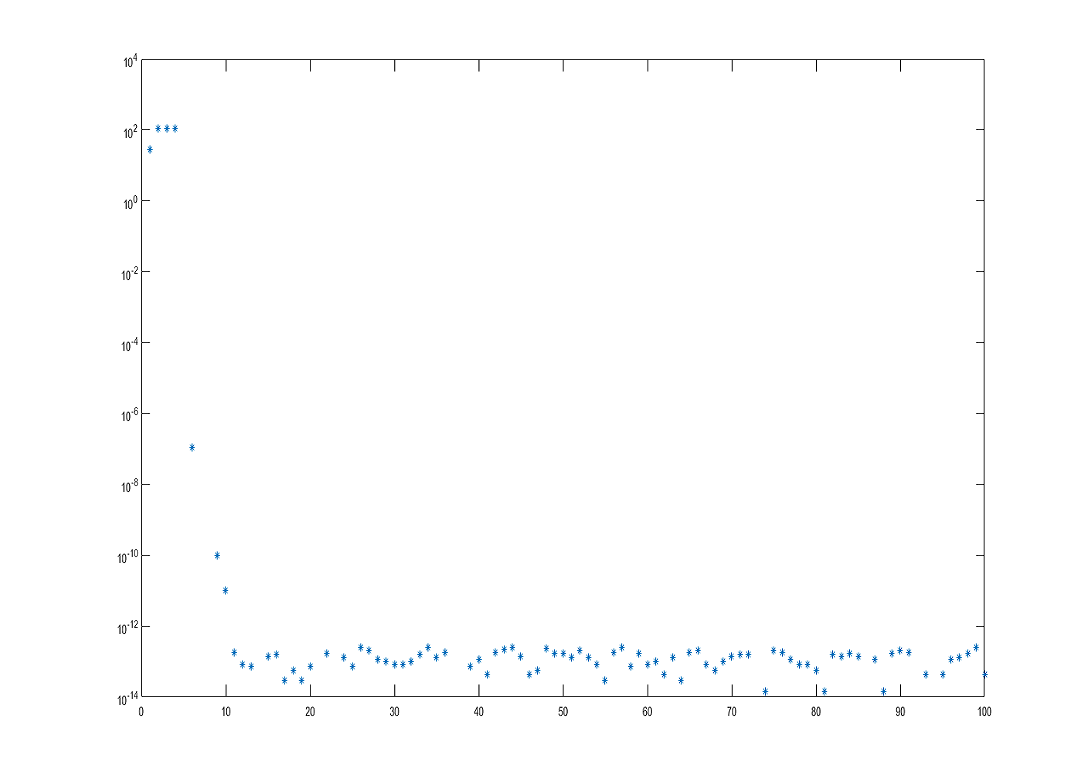
\includegraphics[width=0.5\textwidth]{Tekeningen/arnoldi_1_eig}\label{arnoldi_1_100_it}}
  \hfill
  \subfloat[arnoldi 1, 150 iteraties]{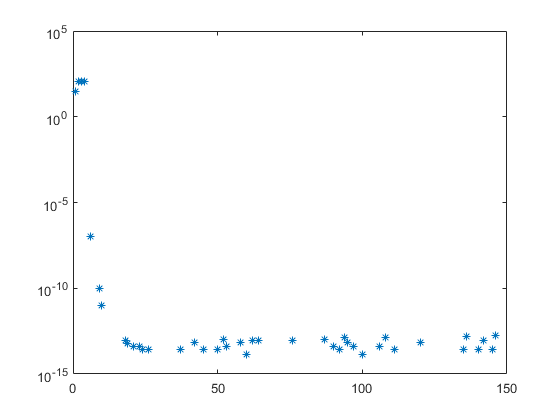
\includegraphics[width=0.5\textwidth]{Tekeningen/arnoldi_1_eig_150it}\label{arnoldi_1_150_it}}
\end{figure}

\begin{figure}[H]
  \centering
  \subfloat[arnoldi 2, 100 iteraties]{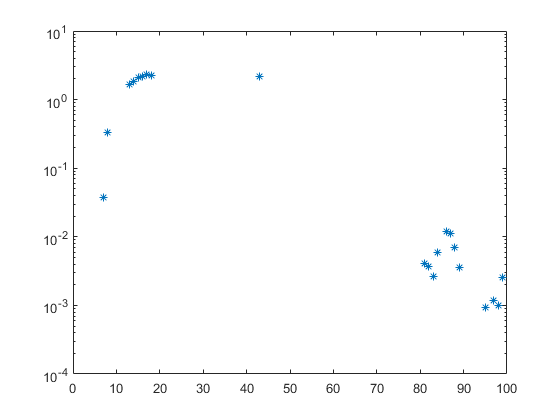
\includegraphics[width=0.5\textwidth]{Tekeningen/arnoldi_2_eig}\label{arnoldi_2_100_it}}
  \hfill
  \subfloat[arnoldi 2, 150 iteraties]{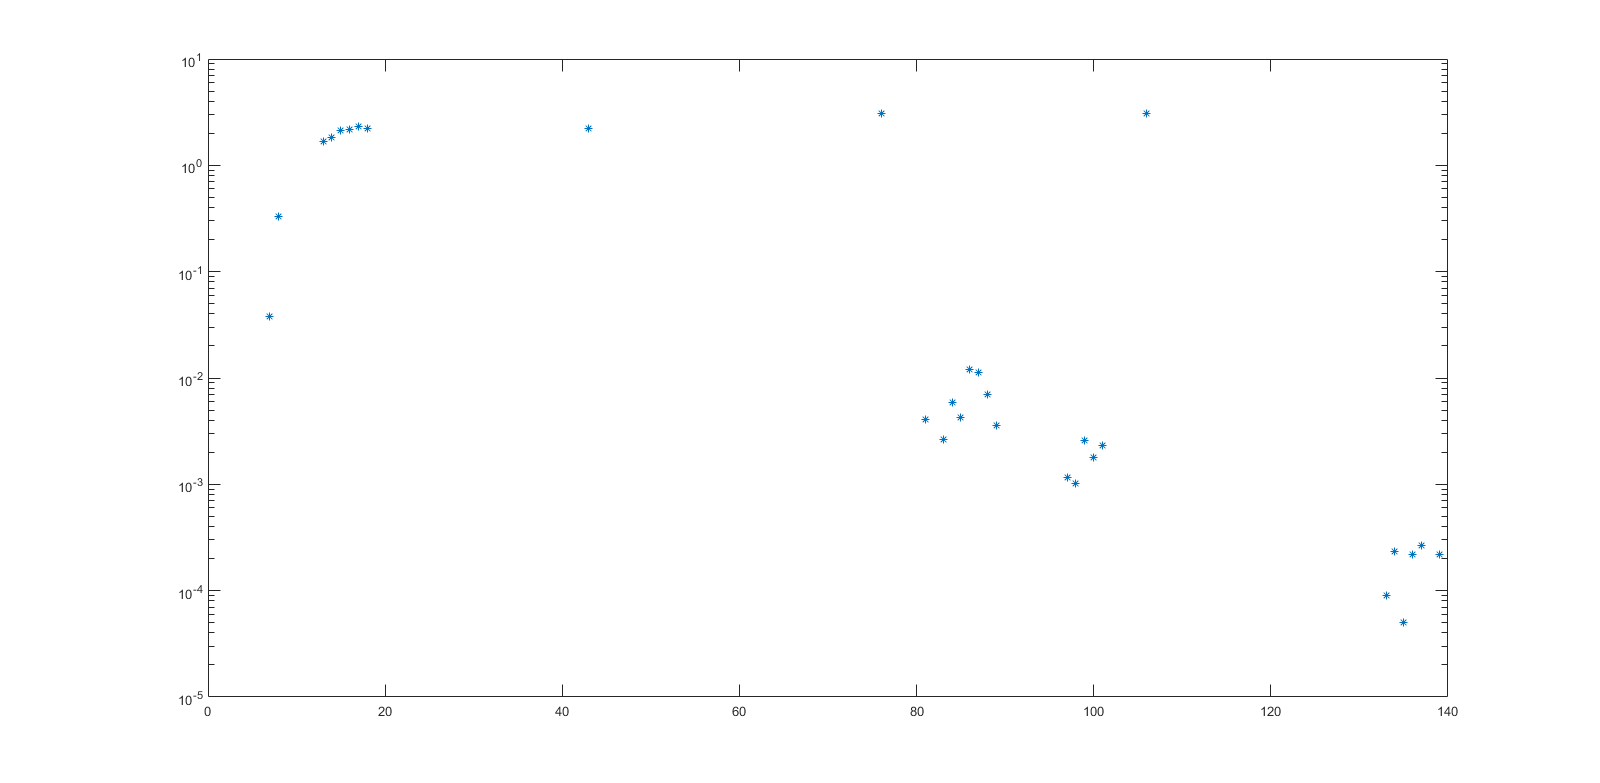
\includegraphics[width=0.5\textwidth]{Tekeningen/arnoldi_2_eig_150it}\label{arnoldi_2_150_it}}
\end{figure}

\begin{figure}[H]
  \centering
  \subfloat[arnoldi 3, 150 iteraties]{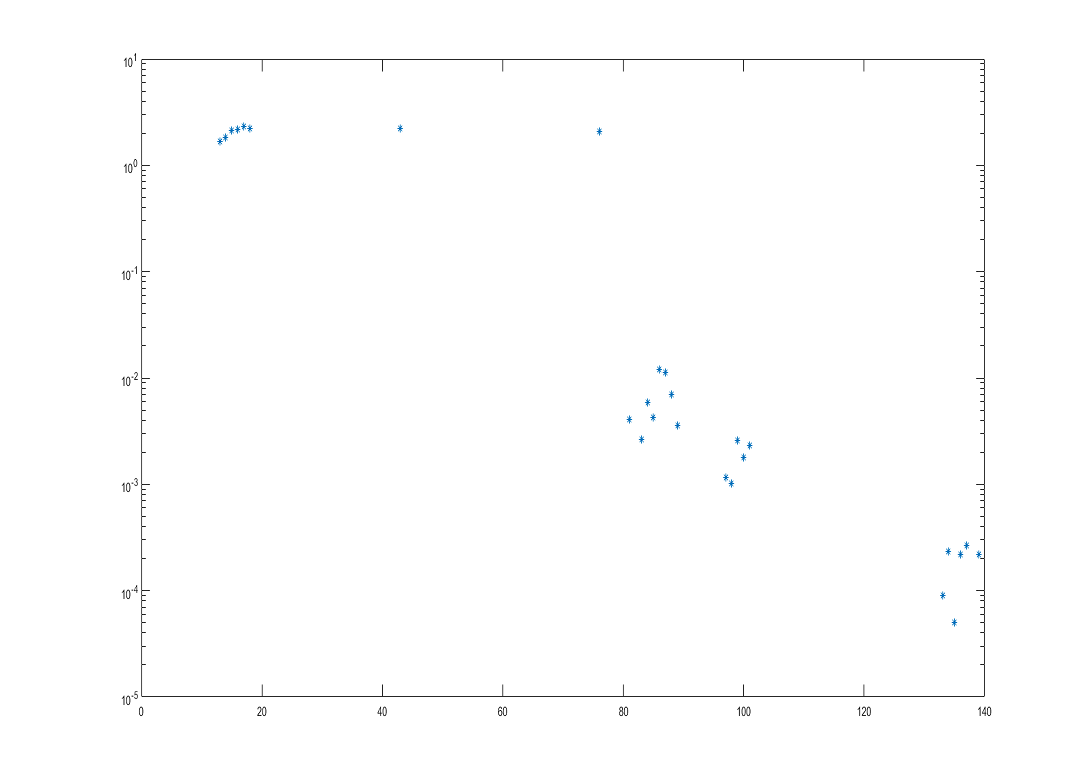
\includegraphics[width=0.5\textwidth]{Tekeningen/arnoldi_3_eig_150it}\label{arnoldi_3_150_it}}
  \hfill
  \subfloat[arnoldi 4, 150 iteraties]{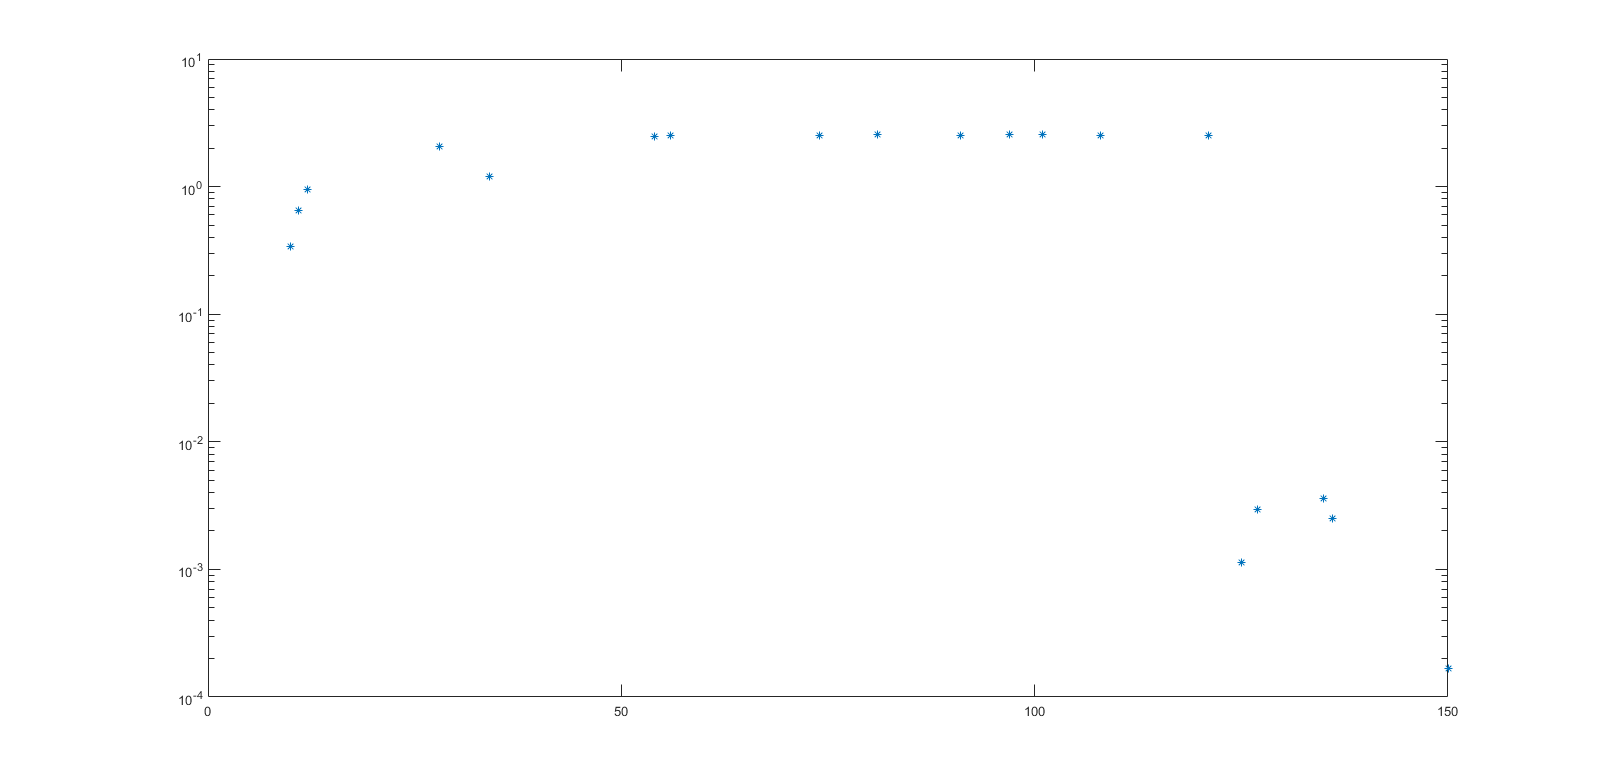
\includegraphics[width=0.5\textwidth]{Tekeningen/arnoldi_4_eig_150i}\label{arnoldi_4_150_it}}
\end{figure}

\opgave{8}
De verschillende $\alpha$ waarden hebben een invloed op de ligging van de eigenwaarden alsook het conditiegetal $\kappa(A)$ van A. Voor $\alpha = 1$ is het conditiegetal $\kappa(A) = 9.4108*10^3$, voor $\alpha = 5$ is $\kappa(A) = 46.6201$, voor $\alpha = 10$ is $\kappa = 13.3134$ en tot slot voor $\alpha = 100$ is $\kappa(A) = 1.5601$.\\[12pt]

Wanneer we nu de eigenwaarden gaan bekijken zien we dat de eigenwaarden bij \ref{alpha 1} het meest verspreid liggen en het meest naar het centrum, hoe hoger de $\alpha$ waarde hoe verder de meeste eigenwaarden zich naar de rand van de eenheidscirkel begeven en dichter bij elkaar komen te liggen. Dit komt ook overeen met de eigenschap:\\
 $\|r_{n}\| \leq inf\|p(A)\| \leq \kappa_{2}(V) inf (max |p(\lambda)|\|r_{0}\|),\forall p\in P_{n}, \forall\lambda\in \sigma(A)$.\\
 Deze stelt immers dat snelle convergentie bereikt wordt voor eigenwaarde van A die geclusterd zitten, weg van de oorsprong en met A gelijkend op een normaal matrix ($A*A^{*} = A^{*}*A$).

\begin{figure}[H]
  \centering
  \subfloat[alpha 1]{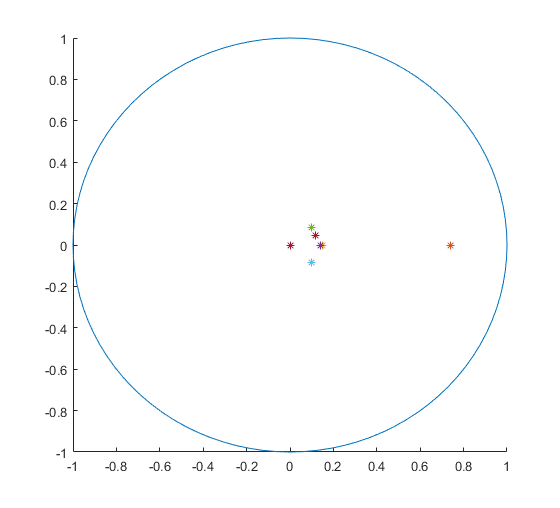
\includegraphics[width=0.5\textwidth]{Tekeningen/GMRES_alpha1_eigenv}\label{alpha 1}}
  \hfill
  \subfloat[alpha 5]{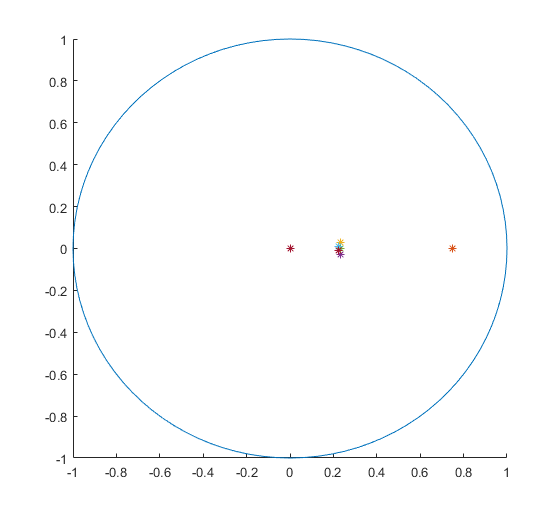
\includegraphics[width=0.5\textwidth]{Tekeningen/GMRES_alpha5_eigenv}\label{alpha 5}}
  \caption{Links eigenwaarden voor $\alpha = 1$, rechts voor $\alpha = 5$}
\end{figure}

\begin{figure}[H]
  \centering
  \subfloat[alpha 10]{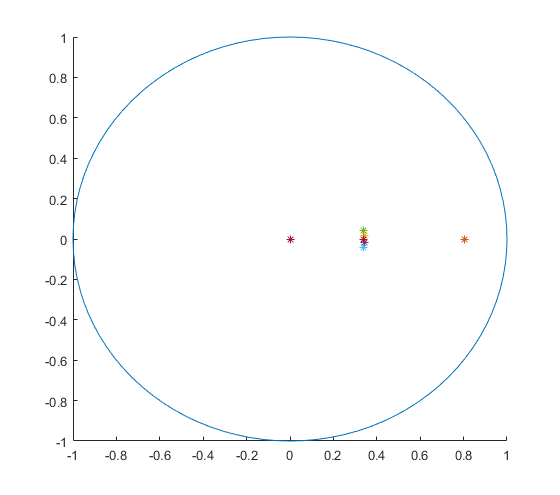
\includegraphics[width=0.5\textwidth]{Tekeningen/GMRES_alpha10_eigenv}\label{alpha 10}}
  \hfill
  \subfloat[alpha 100]{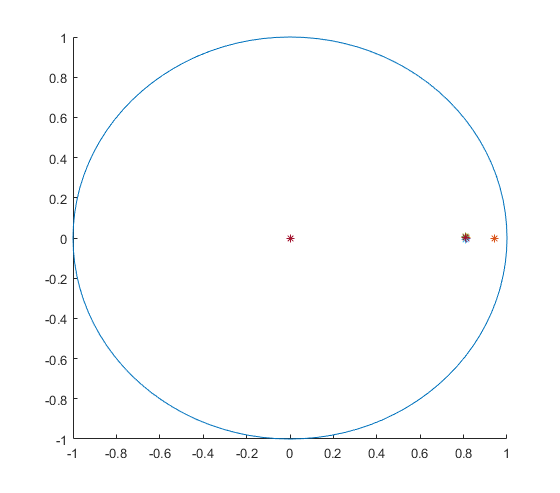
\includegraphics[width=0.5\textwidth]{Tekeningen/GMRES_alpha100_eigenv}\label{alpha 100}}
  \caption{Links eigenwaarden voor $\alpha = 10$, rechts voor $\alpha = 100$}
\end{figure}

\begin{figure}[H]
  \centering
  \subfloat[fout op $\|r_{n}\|$]{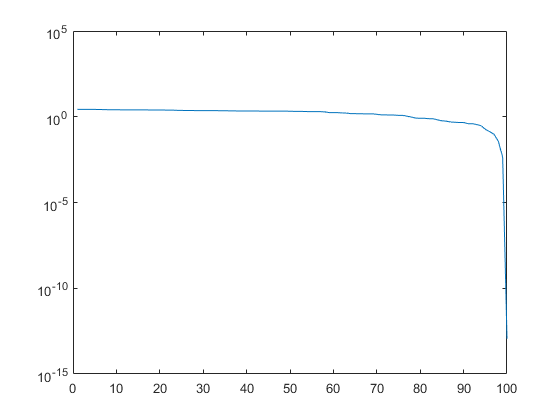
\includegraphics[width=0.5\textwidth]{Tekeningen/GMRES_alpha1_r}\label{r_1}}
  \hfill
  \subfloat[fout op exacte oplossing]{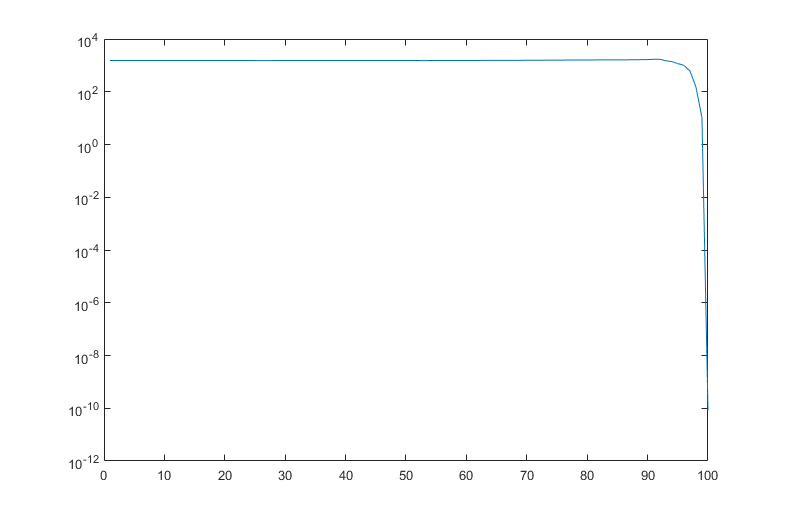
\includegraphics[width=0.5\textwidth]{Tekeningen/GMRES_alpha1_x-y}\label{x-y_1}}
  \caption{Resp. fouten voor $\alpha = 1$.}
\end{figure}

\begin{figure}[H]
  \centering
  \subfloat[fout op $\|r_{n}\|$]{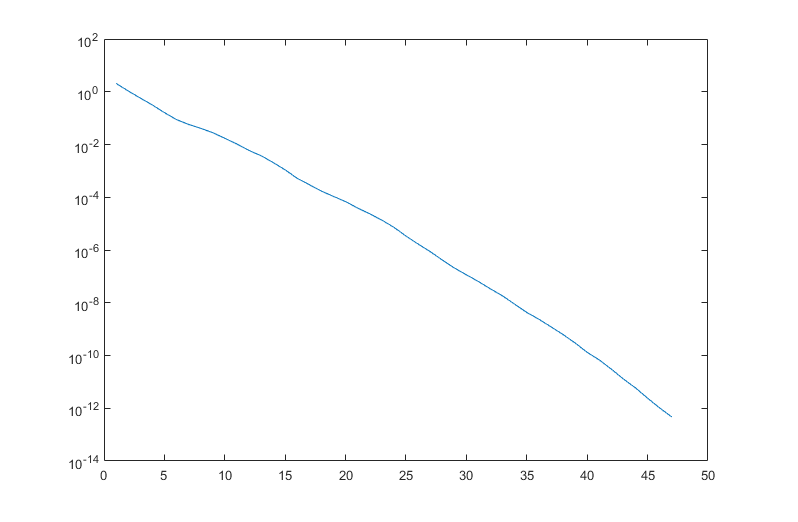
\includegraphics[width=0.5\textwidth]{Tekeningen/GMRES_alpha5_r}\label{r_5}}
  \hfill
  \subfloat[fout op exacte oplossing]{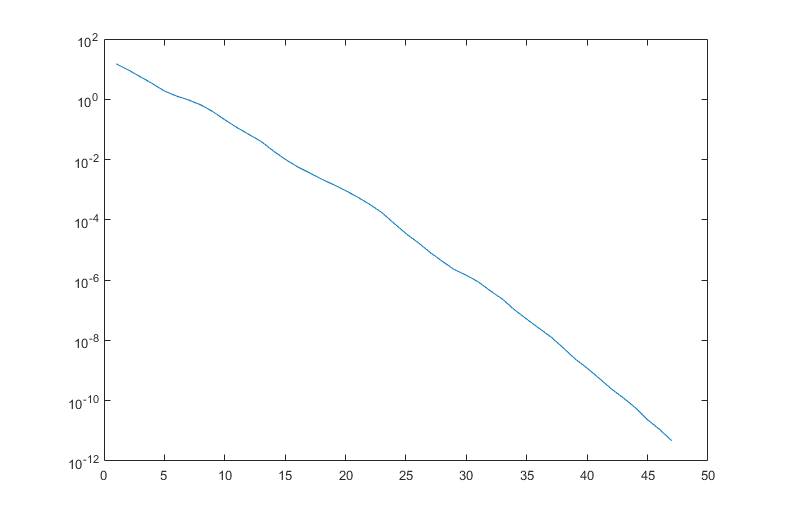
\includegraphics[width=0.5\textwidth]{Tekeningen/GMRES_alpha5_x-y}\label{x-y_5}}
  \caption{Resp. fouten voor $\alpha = 5$.}
\end{figure}

\begin{figure}[!tbp]
  \centering
  \subfloat[fout op $\|r_{n}\|$]{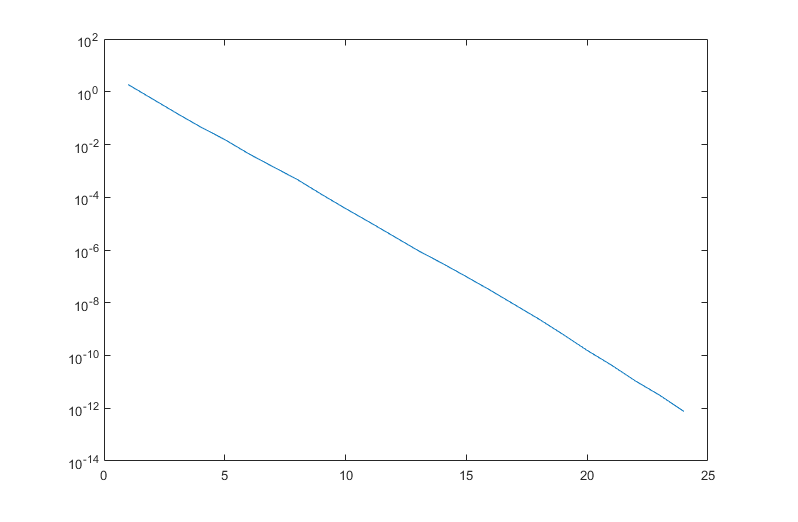
\includegraphics[width=0.5\textwidth]{Tekeningen/GMRES_alpha10_r}\label{r_10}}
  \hfill
  \subfloat[fout op exacte oplossing]{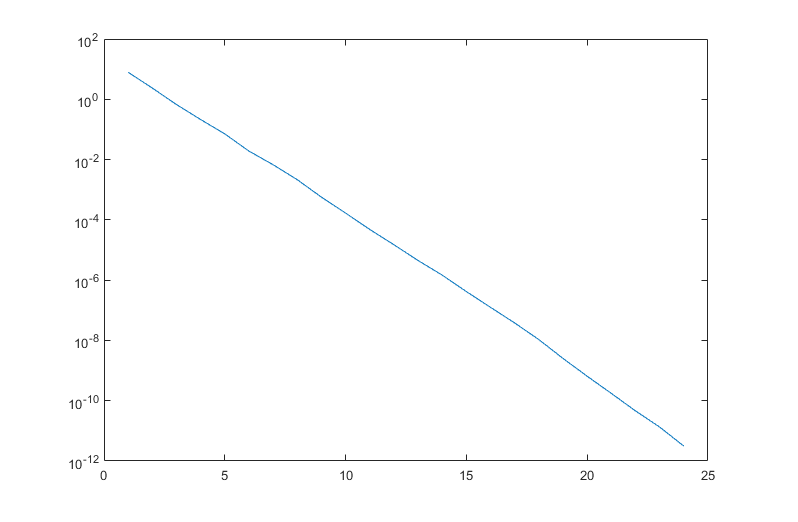
\includegraphics[width=0.5\textwidth]{Tekeningen/GMRES_alpha10_x-y}\label{x-y_10}}
  \caption{Resp. fouten voor $\alpha = 10$.}
\end{figure}

\begin{figure}[!tbp]
  \centering
  \subfloat[fout op $\|r_{n}\|$]{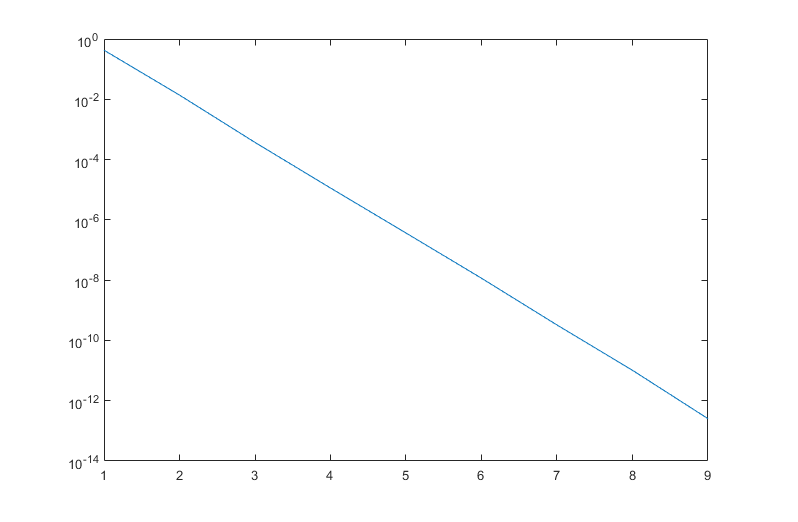
\includegraphics[width=0.5\textwidth]{Tekeningen/GMRES_alpha100_r}\label{r_100}}
  \hfill
  \subfloat[fout op exacte oplossing]{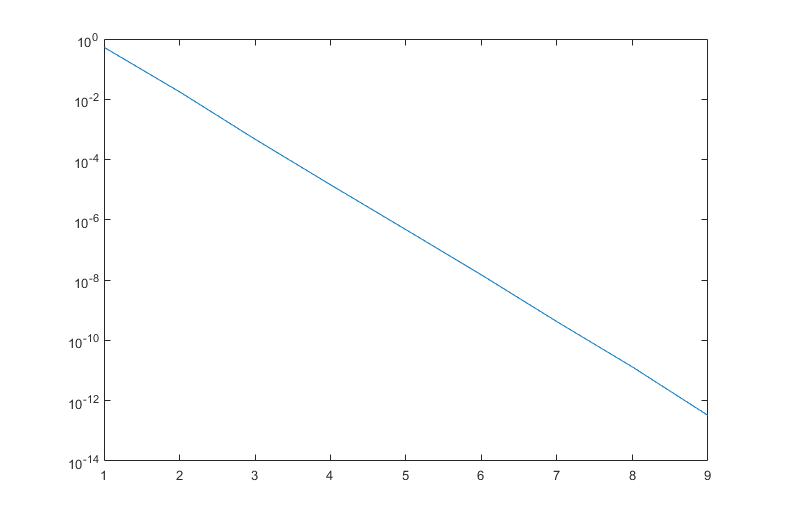
\includegraphics[width=0.5\textwidth]{Tekeningen/GMRES_alpha100_x-y}\label{x-y_100}}
  \caption{Resp. fouten voor $\alpha = 100$.}
\end{figure}




\opgave{9}
De interlacing eigenschap doet een uitspraak over de eigenwaarden van opeenvolgende submatrices van een symmetrische tridiagonaalmatrix A. De formule die geldt is:\\[10pt]

$\lambda_{j}^{(k+1)} < \lambda_{j}^{(k)} < \lambda_{j+1}^{(k+1)}$\\[10pt]

Deze formule stelt dus dat er links en rechts van elke eigenwaarde van submatrix $A^{k}$, steeds een eigenwaarde van de volgende submatrix $A^{(k+1)}$ ligt. Omdat dit geldt voor alle eigenwaarden van $A^{k}$, kan men ook stellen dat er tussen elke twee eigenwaarden j en j+1 van $A^{k}$ er één eigenwaarde ligt van $A^{k+1}$. Om dit grafisch te illustreren, zie de figuur hieronder afkomstig van het boek van Trefethen en Bau.\\

\begin{figure}[H]
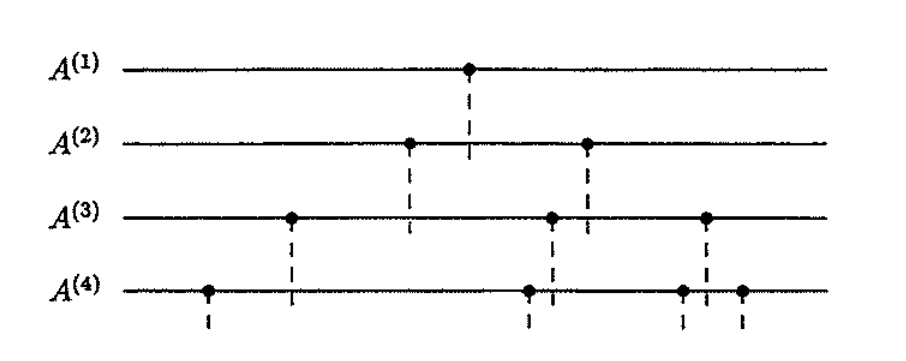
\includegraphics[width=0.8\textwidth]{Tekeningen/Interlacing.png}
  \centering
  \caption{Interlacing eigenschap (Trefethen en Bau, Figure 30.1)}
\end{figure}

Als voorbeeld wordt de volgende matrix gebruikt:\\

\[
A= 
\begin{bmatrix}
    1 & 1 & 0 & 0\\
    1 & 1 & -3 & 0\\
    0 & -3 & 1 & 2\\
    0 & 0 & 2 & 0
\end{bmatrix}
\]\\

De eigenwaarden van de submatrices zijn:\\

$k = 1: \lambda_{0}^{(1)} = 1$\\
$k = 2: \lambda_{0}^{(2)} = 0, \lambda_{1}^{(2)} = 2$\\
$k = 3: \lambda_{0}^{(3)} = -2.1623, \lambda_{1}^{(3)} = 1, \lambda_{2}^{(3)} = 4.1623$\\
$k = 4: \lambda_{0}^{(4)} = -2.8771, \lambda_{1}^{(4)} = 0, \lambda_{2}^{(4)} = 1.2874, \lambda_{3}^{(4)} = 4.5897$\\[10pt]

Voor deze matrix is de interlacing eigenschap dus bevestigd. Deze eigenschap kan dan in de volgende opgave gebruikt worden om de bisectiemethode toe te passen.\\



\opgave{10}
Het algoritme om eigenwaarden te vinden via bisectie is opgedeeld in twee delen. Het eerste deel bepaalt in welk interval er bisectie moet toegepast worden. Het tweede interval past dan echt de bisectie to op het interval. Deel één maakt gebruik van de interlacing eigenschap uit opgave 9. De middengevallen zijn het makkelijkst op te stellen. Het interval is dan tussen twee opeenvolgende eigenwaarden van $A^{(k)}$. Bisectie wordt dan toegepast op de karakteristieke veelterm van $A^{(k+1)}$. Aan de randen wordt dan gekeken tussen de dichtsbijzijnde eigenwaarde in het interval en de rand van het interval.\\

Als makkelijk bestudeerbaar geval werd er gekozen voor de matrix uit opgave 9. Dit is een relatief kleine matrix en dus makkelijk om te overzien. Als eerste werd er gekozen voor een interval dat alle eigenwaarden omvat (-3, 5). De methode was dan in staat om alle eigenwaarden te vinden. Vervolgens werd er een kleiner interval gekozen, zodat niet alle eigenwaarden gevonden konden worden. Ook bij deze test slaagde het programma erin om alle eigenwaarden van A binnen het interval te berekenen. Bij een interval zonder eigenwaarden, werden er ook geen teruggegeven.\\

De belangerlijkste eigenschappen die een matrix A moet bezitten om getest te kunnen worden, waren tridiagonaliteit en symmetrie. Dit zorgt voor de interlacing eigenschap. En deze zorgt weer voor een gebrek aan dubbele nulpunten. Een andere matrix waarop getest werd, was:\\

\[
A = 
\begin{bmatrix}
1&	-2&	0	&0	&0	&0&	0	&0&	0&	0\\
-2	&1&	-2	&0&	0&	0&	0&	0&	0&	0\\
0	&-2&	1	&-2	&0	&0&	0&	0&	0&	0\\
0&	0&	-2	&1&	-2	&0&	0	&0	&0&	0\\
0&	0	&0&	-2	&1&	-2&	0&	0&	0&	0\\
0	&0&	0	&0	&-2	&1&-2&	0&	0&	0\\
0	&0&	0&	0&	0&	-2&	1	&-2	&0&	0\\
0	&0	&0&	0&	0&	0&	-2&	1&	-2&	0\\
0&	0	&0&	0&	0&	0&	0&	-2&	1	&-2\\
0&	0	&0&	0	&0	&0	&0	&0	&-2&	1
\end{bmatrix}
\]\\

Deze matrix is opnieuw symmetrisch en tridiagonaal, maar heeft niet bepaald interessante eigenwaarden. Hij werd gewoon gebruikt om de correctheid na te gaan. De testen werden wel interessant wanneer er vrij grote matrices werden gebruikt. Een essenti\"ele eigenschap voor de bisectiemethode is de interlacing eigenschap zoals beschreven in opgave 9. Wanneer er bijvoorbeeld een 1000x1000 matrix werd aangemaakt, doken er hier problemen op. De interlacing eigenschap zegt dat eigenwaarden van $A^{(k)}$ nooit gelijk kunnen zijn aan deze van $A^{(k-1)}$. Echter bij het berekenen van grote matrices, werd het verschil in eigenwaarden van deze twee matrices te klein. Daardoor werkte de bisectiemethode niet meer. Het vergroten van een $A^{(998)}$ naar een $A^{(999)}$ zorgde voor een niet waarneembaar verschil op de eerste eigenwaarde.\\




\begin{algorithm}[ht!]
	\caption{\texttt{Bisectie\_intervalbepaling}}
	\label{Bisectie_intervalbepaling}
	\begin{algorithmic}[1]
		\Procedure{bisection\_eigenvalue}{A, a, b, tol}
		\For{k van 1 tot aantal rijen A}{}
			\State Bereken de karakteristieke veelterm van $A^{(k)}$
			\State Initialiseer nieuwe E
			\For{j van 1 tot aantal eigenwaarden in $A^{(k-1)}$ + 1}
			\If{j gelijk aan maximum}
				\State $\lambda =$ bisection(p(A), a\_new, b, tol)
				\State Voeg $\lambda$ toe aan E	
			\Else
				\State $\lambda =$  bisection(p(A), a\_new, E\_old(1,j), tol)
				\State a\_new = E\_old(1,j)
				\State Voeg $\lambda$ toe aan E
			\EndIf
			\EndFor
			\State $E\_old = E$
		\EndFor
		\State \Return{E}
		\EndProcedure
	\end{algorithmic}
\end{algorithm}

\begin{algorithm}[ht!]
	\caption{\texttt{Bisectie}}
	\label{Bisectie}
	\begin{algorithmic}[1]
		\Procedure{bisection}{p, a, b, tol}
		\While{abs(a-b) $\leq$ tol}
			\State Bereken fa =p(a) en fb = p(b)
			\If{fa*fb $>$ 0}
				\State In dit geval is er geen nulpunt in het interval.
				\State \Return{Lege lijst}
			\Else
				\State Stel $x = (a+b)/2$
				\State Bereken fx
			\If{$fx = 0$ of kleiner dan tol}
				\State Stel a en b gelijk aan x
			\ElsIf{fa*fx $<$ 0}
				\State Stel b gelijk aan x, want nulpunt in linkse interval.
			\Else
				\State Stel a gelijk aan x, want nulpunt rechtse interval.
			\EndIf
			\EndIf
		\EndWhile
		\State \Return{x}
		\EndProcedure
	\end{algorithmic}
\end{algorithm}

\section*{Bijlage 1}
\begin{landscape}
\begin{table}[htb]
\centering
\caption{Resultaten Opgave 3}
\label{Kleinste Kwadraten}
\resizebox{2\textwidth}{!}{\begin{tabular}{|l|l|l|l|l|l|l|l|l|l|l|l|l|l|l|l|l|l|l|l|l|l|l|l|l|l|l|l|l|l|l|l|}
\hline
n & \multicolumn{30}{l|}{x}      & Residu \\ \hline
0 & Empty & & & & & & & & & & & & & & & & & & & & & & & & & & & & & & 99.354\\ \hline
1 & 0.4006 & & & & & & & & & & & & & & & & & & & & & & & & & & & & & & 99.026\\ \hline
2 & 0.4006 & 0.7361 & & & & & & & & & & & & & & & & & & & & & & & & & & & & & 97.9037\\ \hline
3 & 0.4081 &-0.7350 & 0.8591 & & & & & & & & & & & & & & & & & & & & & & & & & & & & 96.3868 \\ \hline
4 & 0.5359 &-0.7057 &0.8436 &2.6204 & & & & & & & & & & & & & & & & & & & & & & & & & & & 81.0928  \\ \hline
5 & 0.5594 &-0.6631 &0.8374 &2.6316 &0.6548& & & & & & & & & & & & & & & & & & & & & & & & & & 79.9244  \\ \hline
6 & 0.5466 &-0.6671 &0.8238 &2.6353 &0.6495 &-0.1635 & & & & & & & & & & & & & & & & & & & & & & & & & 79.8340   \\ \hline
7 & 0.5297 &-0.7178 &0.7779 &2.5840 &0.6505 &-0.1741 &-0.9020 & & & & & & & & & & & & & & & & & & & & & & & & 77.7808    \\ \hline
8 &0.5232 &-0.7113 &0.7993 &2.6052 &0.6740 &-0.1759 &-0.8986 &0.4034& & & & & & & & & & & & & & & & & & & & & & & 77.3647     \\ \hline
9 &0.5299 &-0.7260 &0.8094 &2.6487 &0.7083 &-0.1249 &-0.9047 &0.4121 &0.7658 & & & & & & & & & & & & & & & & & & & & & & 75.7822     \\ \hline
10 &0.5507 &-0.7184 &0.7986 &2.6572 &0.7470 &-0.0906 &-0.8561 &0.4045 &0.7753 &0.6939 & & & & & & & & & & & & & & & & & & & & & 74.4638     \\ \hline
11 &0.5640 &-0.7032 &0.8049 &2.6494 &0.7529 &-0.0620 &-0.8347 &0.4417 &0.7668 &0.7014 &0.4885& & & & & & & & & & & & & & & & & & & & 73.7752      \\ \hline
12 &0.5084 &-0.7113 &0.7901 &2.6645 &0.7452 &-0.1100 &-0.8770 &0.3654 &0.6990 &0.6868 &0.5009 &-1.2303 & & & & & & & & & & & & & & & & & & & 69.6450      \\ \hline
13 &0.4595 &-0.6609 &0.7938 &2.6786 &0.7306 &-0.1080 &-0.8355 &0.4085 &0.7689 &0.7477 &0.5168 &-1.2477 &1.1707 & & & & & & & & & & & & & & & & & & 65.6946       \\ \hline
14 &0.4311 &-0.6403 &0.7474 &2.6674 &0.7116 &-0.1125 &-0.8319 &0.3903 &0.7265 &0.7064 &0.4679 &-1.2527 &1.1754 &-0.7924 & & & & & & & & & & & & & & & & & 63.8362        \\ \hline
15 &0.4600 &-0.6741 &0.7719 &2.6351 &0.7108 &-0.1241 &-0.8302 &0.3898 &0.7029 &0.6748 &0.4267 &-1.2907 &1.1645 &-0.7819 &-0.7122 & & & & & & & & & & & & & & & & 62.3017         \\ \hline
16 &0.4043 &-0.7052 &0.8122 &2.6023 &0.7436 &-0.1229 &-0.8158 &0.3854 &0.7060 &0.7036 &0.4609 &-1.2431 &1.2085 &-0.7690 &-0.7197 &0.8266 & & & & & & & & & & & & & & & 60.1877         \\ \hline
17 &0.3225 &-0.6070 &0.8576 &2.5276 &0.8042 &-0.1834 &-0.8199 &0.3678 &0.7151 &0.6893 &0.4096 &-1.3057 &1.1279 &-0.8479 &-0.7466 &0.8455 &-1.4350& & & & & & & & & & & & & & 53.2508 \\ \hline
18 &0.3137 &-0.6066 &0.8591 &2.5435 &0.8058 &-0.1894 &-0.8422 &0.3543 &0.6996 &0.6757 &0.4193 &-1.3024 &1.1016 &-0.8478 &-0.7711 &0.8560 &-1.4468 &-0.2232 & & & & & & & & & & & & & 52.8676 \\ \hline
19 &0.2887 &-0.6052 &0.8703 &2.5247 &0.7852 &-0.1803 &-0.8500 &0.3826 &0.7111 &0.6893 &0.4285 &-1.3098 &1.1079 &-0.8170 &-0.7585 &0.8896 &-1.4534 &-0.2164 &0.4211  & & & & & & & & & & & & 52.1452  \\ \hline
20 &0.2500 &-0.6233 &0.8504 &2.5599 &0.7357 &-0.2033 &-0.8181 &0.3499 &0.7363 &0.6885 &0.4331 &-1.3202 &1.1165 &-0.7961 &-0.7306 &0.9267 &-1.4222 &-0.2035 &0.4125 &0.6705 & & & & & & & & & & & 50.4700  \\ \hline
21 &0.2551 &-0.6267 &0.8583 &2.5561 &0.7381 &-0.2049 &-0.8129 &0.3529 &0.7326 &0.6812 &0.4284 &-1.3256 &1.1109 &-0.7915 &-0.7289 &0.9182 &-1.4202 &-0.2116 &0.4175 &0.6651 &-0.0535 & & & & & & & & & & 50.4245   \\ \hline
22 &0.2664 &-0.6420 &0.8846 &2.5663 &0.7548 &-0.2308 &-0.7808 &0.3673 &0.7093 &0.7030 &0.4126 &-1.3237 &1.1078 &-0.7820 &-0.7390 &0.9006 &-1.4375 &-0.2390 &0.4000 &0.6562 &-0.0453 &-0.4515 & & & & & & & & & 49.6277    \\ \hline
23 &0.2637 &-0.6324 &0.8724 &2.5876 &0.7618 &-0.2158 &-0.8017 &0.3932 &0.7216 &0.6844 &0.4303 &-1.3354 &1.1091 &-0.7835 &-0.7300 &0.8929 &-1.4514 &-0.2534 &0.3766 &0.6417 &-0.0524 &-0.4434 &-0.3701& & & & & & & & 49.0799  \\ \hline
24 &0.2530 &-0.6399 &0.8760 &2.5996 &0.7463 &-0.2080 &-0.8133 &0.4057 &0.7077 &0.6874 &0.4426 &-1.3494 &1.1041 &-0.7911 &-0.7368 &0.8822 &-1.4413 &-0.2458 &0.3709 &0.6555 &-0.0579 &-0.4326 &-0.3813 &0.0830 & & & & & & & 48.9233  \\ \hline
25 &0.2447 &-0.6347 &0.8857 &2.5908 &0.7381 &-0.2020 &-0.8243 &0.4106 &0.7044 &0.6908 &0.4338 &-1.3539 &1.1106 &-0.7804 &-0.7288 &0.8915 &-1.4335 &-0.2531 &0.3692 &0.6680 &-0.0612 &-0.4194 &-0.3894 &0.0911 &0.0823 & & & & & & 48.8153  \\ \hline
26 &0.2345 &-0.6228 &0.8766 &2.5823 &0.7437 &-0.1916 &-0.8360 &0.4200 &0.6955 &0.6994 &0.4243 &-1.3493 &1.1207 &-0.7921 &-0.7357 &0.8842 &-1.4426 &-0.2618 &0.3784 &0.6736 &-0.0705 &-0.4095 &-0.3985 &0.1012 &0.0718 &0.0164 & & & & & 48.7040  \\ \hline
27 &0.2492 &-0.6322 &0.8922 &2.5700 &0.7387 &-0.1891 &-0.8229 &0.4024 &0.7023 &0.6854 &0.4393 &-1.3653 &1.1202 &-0.7756 &-0.7539 &0.8802 &-1.4495 &-0.2699 &0.3683 &0.6839 &-0.0609 &-0.4151 &-0.3807 &0.0974 &0.0835 &0.0040 &0.1366 & & & & 48.4935  \\ \hline
28 &0.2473 &-0.6318 &0.8895 &2.5706 &0.7387 &-0.1920 &-0.8199 &0.4032 &0.7031 &0.6887 &0.4399 &-1.3666 &1.1219 &-0.7724 &-0.7546 &0.8811 &-1.4529 &-0.2712 &0.3658 &0.6825 &-0.0599 &-0.4156 &-0.3849 &0.0959 &0.0789 &0.0052 &0.1354 &-0.0569& & & 48.4793  \\ \hline
29 &0.2375 &-0.6360 &0.8783 &2.5871 &0.7241 &-0.1840 &-0.8041 &0.3880 &0.6912 &0.6979 &0.4210 &-1.3600 &1.1168 &-0.7681 &-0.7680 &0.8744 &-1.4434 &-0.2548 &0.3766 &0.6993 &-0.0463 &-0.4263 &-0.3895 &0.1175 &0.0738 &0.0265 &0.1211 &-0.0446 &0.1485 & & 48.1917 \\ \hline
30 & 0.2170&-0.6298&0.8726&2.5880&0.7125&-0.1795&-0.8057&0.3754&0.7041&0.7022&0.4211&-1.3469&1.1179&-0.7712&
-0.7625&0.8886&-1.4458&-0.2534&0.3643&0.6943&-0.0563&-0.4316&-0.3870&0.1183&0.0574&0.0210&0.1031&-0.0399&0.1444&-0.2004&48.0000  \\ \hline
\end{tabular}}
\end{table}
\end{landscape}

\end{flushleft}
\end{document}